\documentclass[11pt,letter]{ivoa}
\input tthdefs


\usepackage{listings}
\usepackage{relsize}
\lstloadlanguages{XML,HTML}
\lstset{flexiblecolumns=true,basicstyle=\small,tagstyle=\ttfamily,
  showstringspaces=False}
\usepackage[utf8]{inputenc}

\hyphenation{asyn-chro-n-ous-ly}

\title{Table Access Protocol}

\ivoagroup{Data Access Layer Working Group}

\author{Patrick Dowler, Guy Rixon, Doug Tody, Markus Demleitner}

\editor{Patrick Dowler}

\previousversion[http://www.ivoa.net/Documents/TAP/20190826/]{PR-TAP-1.1-20190826}
\previousversion[http://www.ivoa.net/Documents/TAP/20190626/]{PR-TAP-1.1-20190626}
\previousversion[http://www.ivoa.net/Documents/TAP/20190420/]{PR-TAP-1.1-20190420}
\previousversion[http://www.ivoa.net/Documents/TAP/20181024/]{PR-TAP-1.1-20181024}
\previousversion[http://www.ivoa.net/Documents/TAP/20180830/]{PR-TAP-1.1-20180830}
\previousversion[http://www.ivoa.net/Documents/TAP/20180416/]{PR-TAP-1.1-20180416}
\previousversion[http://www.ivoa.net/Documents/TAP/20170830/]{PR-TAP-1.1-20170830}
\previousversion[http://www.ivoa.net/Documents/TAP/20170707/]{WD-TAP-1.1-20170707}
\previousversion[http://www.ivoa.net/Documents/TAP/20160428/]{WD-TAP-1.1-20160428}
\previousversion[http://www.ivoa.net/Documents/TAP/1.0]{TAP-1.0}


\iftth
\newcommand{\tapschema}{TAP\_SCHE\-MA}
\hyphenation{TAP\_SCHEMA}
\hyphenation{\tapschema}
\newcommand{\tapupload}{TAP\_UPLOAD}
\else
\newcommand{\tapschema}{\mbox{%
  \relsize{-0.5}TAP\discretionary{-}{}{\kern-2pt\_}SCHEMA}}
\newcommand{\tapupload}{%
  {\relsize{-0.5}TAP\discretionary{-}{}{\kern-2pt\_}UPLOAD}}
\fi

\begin{document}

\begin{abstract}
The table access protocol (TAP) defines a service protocol for accessing general 
table data, including astronomical catalogs as well as general database tables. 
Access is provided for both database and table metadata as well as for actual 
table data. This version of the protocol includes support for multiple query 
languages, including queries specified using the Astronomical Data Query 
Language ADQL  within an integrated interface. It also includes 
support 
for both synchronous and asynchronous queries. Special support is provided for
spatially indexed queries using the spatial extensions in ADQL. A multi-position 
query capability permits queries against an arbitrarily large list of 
astronomical targets, providing a simple spatial cross-matching capability. 
More sophisticated distributed cross-matching capabilities are possible by 
orchestrating a distributed query across multiple TAP services.  
\end{abstract}


\section*{Acknowledgments}

The authors would like to acknowledge all contributors to this and previous 
versions of this standard, especially: K. Andrews, J. Good, R. Hanisch, G. 
Lemson, T. McGlynn, K. Noddle, F. Ochsenbein, I. Ortiz, P. Osuna, R. Plante, 
J. Salgado, A. Stebe, and A. Szalay.


\section*{Conformance-related definitions}

The words ``MUST'', ``SHALL'', ``SHOULD'', ``MAY'', ``RECOMMENDED'', and
``OPTIONAL'' (in upper or lower case) used in this document are to be
interpreted as described in IETF standard, \citet{std:RFC2119}.

The \emph{Virtual Observatory (VO)} is general term for a collection of 
federated resources that can be used to conduct astronomical research, 
education, and outreach. The \href{http://www.ivoa.net}{International
Virtual Observatory Alliance (IVOA)} is a global collaboration of separately 
funded projects to develop standards and infrastructure that enable VO 
applications.


\section{Introduction}
\label{sec:Introduction}

The Table Access Protocol (TAP) is a web-service protocol that gives access to 
collections of tabular data referred to collectively as a tableset.  TAP 
services accept queries posed against the tableset available via the service and 
return the query response as another table, in accord with the relational model. 
 Queries may be submitted using various query languages and may execute 
synchronously or asynchronously. Support for the Astronomical Data Query 
Language ADQL \citep{2008ivoa.spec.1030O} is mandatory; support for other query languages is 
supported 
but optional.

The result of a TAP query is another table, normally returned as a VOTable. 
Support for VOTable output is mandatory; all other formats are optional.

The table collections made accessible via TAP are typically stored in relational 
database management systems (RDBMS). A TAP service exposes the database schema 
to client applications so that queries can be posed directly against arbitrary 
data tables available via the service.

Multi-table operations such as joins or cross matches are possible provided the 
tables are all managed by the local TAP service, and provided the service 
supports these capabilities.  Larger scale operations such as a distributed 
cross match are also possible, but require combining the results of multiple TAP 
services.

\subsection{Role within the VO Architecture}
\label{sec:Role}

% NOTE: not in TAP-1.0

\begin{figure}
\centering

% Get the architecture diagram from the TCG chair
% http://wiki.ivoa.net/twiki/bin/view/IVOA/IvoaTCG
% If they give you a PDF, for now dumb it down to a png by
% convert -antialias -density 72x72 archdiag.pdf archdiag.png
% Oh -- Notes don't need this; you'd have to remove archdiag.png
% from FIGURES in the Makefile, too.

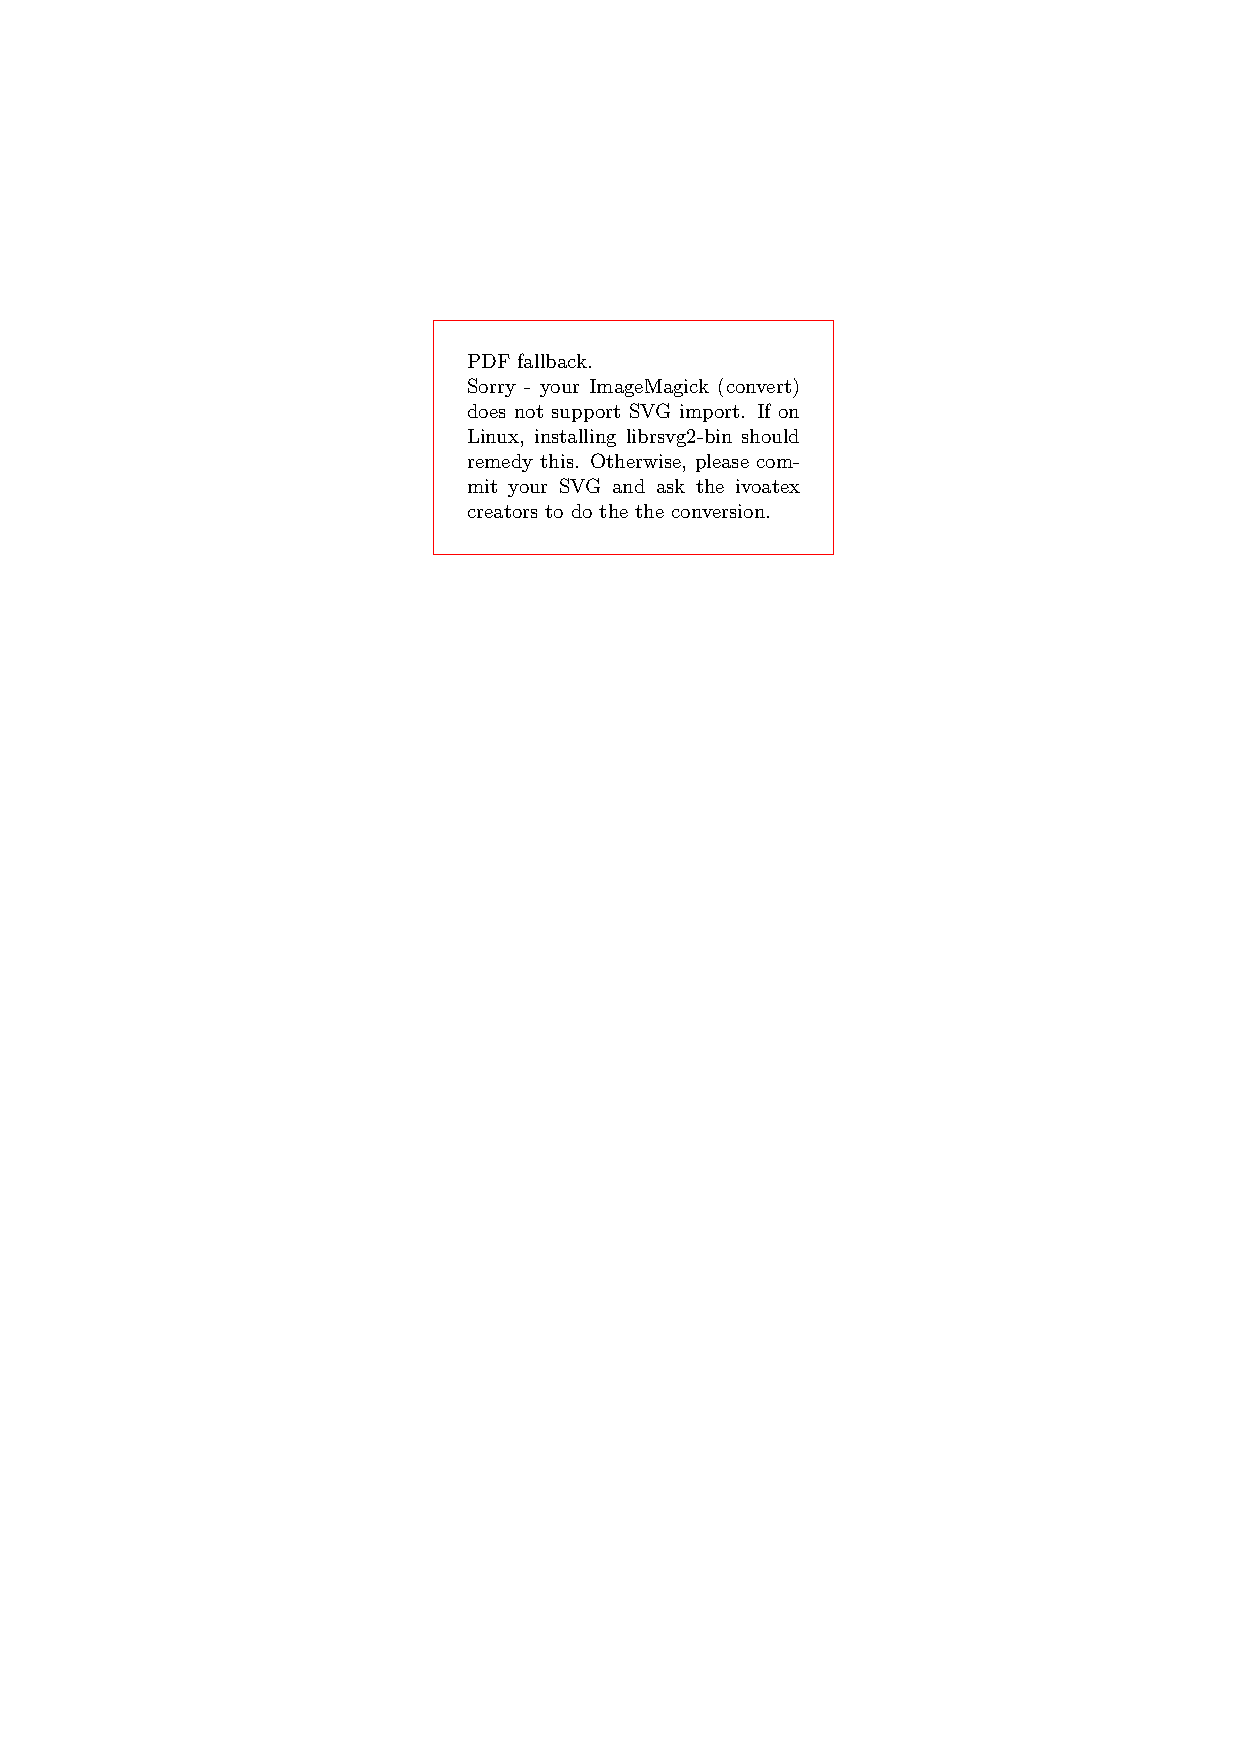
\includegraphics[width=0.9\textwidth]{role_diagram.pdf}
\caption{Architecture diagram for this document}
\label{fig:archdiag}
\end{figure}

Fig.~\ref{fig:archdiag} shows the role this document plays within the
IVOA architecture \citep{note:VOARCH}.

TAP depends on the following other IVOA standards:

\begin{description}

\item[UWS \citep{2016ivoa.spec.1024H}] TAP services can be queried
asynchronously; the Universal Worker Service UWS defines the
corresponding communication pattern.  Note that while TAP 1.1 does not
require the use of any particular minor version of the UWS standard, 
UWS 1.1 can significantly streamline the communication, and
implementors of TAP 1.1 are encouraged to support UWS 1.1 or later.

\item[ADQL \citep{2008ivoa.spec.1030O}] A standards-compliant TAP
service must support queries written in the Astronomical Data Query
Language.

\item[VOSI \citep{2017ivoa.spec.0524G}] The VO Support Interfaces standard
defines endpoints for metadata discovery; for TAP, this is the tables,
capabilities, and availability endpoints. Note that while TAP 1.1 does not
require the use of any particular minor version of the VOSI standard, 
the VOSI-tables resource in VOSI 1.1 provides important usability features, and
implementors of TAP 1.1 are encouraged to support VOSI 1.1 or later.

\item[VOTable \citep{2013ivoa.spec.0920O}] All TAP services must be able
to serve query results in the VOTable format. Note that while TAP 1.1 does not
require the use of any particular minor version of the VOTable standard, older 
versions are missing features that are required and may be unusable in practice.
For example, the overflow reporting and xtype attribute were introduced in 
VOTable 1.2 so that is the minimum viable version that must be used.

\item[SSO \citep{2017ivoa.spec.0524T}] TAP services that support authenticated 
access declare this in their capabilities using recommendations and security method 
identifiers from the SSO standard.
\end{description}


TAP is related in other ways to the following IVOA standards:

\begin{description}
\item[DALI \citep{2017ivoa.spec.0517D}]  The Data Access Layer Interface standard
gives general rules for the construction of DAL standards.  TAP has been
written against version 1.1 of DALI.  In particular, TAP directly
references DALI 1.1's serialisation rules for geometries and timestamps
and recommends implementing the examples endpoint defined by DALI.

\item[Obscore \citep{2017ivoa.spec.0509L}] The Obscore data model
facilitates the publication of metadata of observational data products.
TAP is used to access compliant metadata collections.

\item[RegTAP \citep{2014ivoa.spec.1208D}]  The relational model for the
VO Registry provides a data model for publishing service metadata.
TAP is used to access compliant metadata collections.

\item[TAPRegExt \citep{2012ivoa.spec.0827D}] While there is no formal
requirement to that effect, the response on a TAP service's capabilities
endpoint should contain instances of \xmlel{tr:TableAccess}-typed
capabilities in order to allow clients to discover several important
aspects of a TAP service's capabilities (e.g., resource limits, output
formats, user defined functions).

\item[CDP \citep{2010ivoa.spec.0218P}] TAP services that support authenticated requests may require 
delegation of user credentials in order for some features to work; such services
will have an associated credential service and could use delegated credentials for 
remote calls that require authentication. For example, a URL specified in the UPLOAD
parameter may require authentication and the service would use delegated credentials
to perform the retrieval.
\end{description}

\subsection{Motivating Use Cases}
Below are some of the more common use cases that have motivated the development 
of the TAP specification. While this is not complete, it helps to understand the 
problem area covered by this specification.

\subsubsection{Discover Metadata}
Since content in relational databases is often custom and project-specific, 
users of a TAP service must be able to discover the names of tables and 
columns, datatypes, units, and other information necessary to construct 
meaningful correct queries.

\subsubsection{Query Custom Tables}
A large amount of astronomical data and metadata is stored in tables in 
relational databases. Historically, users could query these tables through 
custom user interfaces (usually web page forms), but such approaches could not 
provide support for truly ad-hoc querying. A TAP service should enable users to 
discover and query custom tables with a flexible and expressive input that 
supports ad-hoc querying: selecting output, filtering the result, joining 
multiple tables, computing aggregate quantities, etc. 

\subsubsection{Query Standard Tables}
A TAP service should enable users to query externally defined standard tables 
in a uniform way such that the same web service request can be sent to multiple 
services. Services must be able to declare their support for standard tables in 
the service metadata.

\subsubsection{Query Standard Data Models}
A TAP service should enable users to query (parts of) externally defined data 
models that are (partially or fully) implemented by the service. Services must 
be able to declare their support for data models as well as the way those model 
elements are mapped to tables and columns.

\subsection{Query Languages}

\subsubsection{ADQL Queries}
The Astronomical Data Query Language ADQL \citep{2008ivoa.spec.1030O} is the standard 
query language for the IVOA. Support for ADQL queries is mandatory. ADQL can be 
used to specify queries  that access one or more tables provided by the TAP 
service, including the standard metadata tables. In general, the client must 
access table metadata in order to discover the names of tables and columns and 
then formulate queries. ADQL queries provide a direct (low-level) access to the 
tables; a query will be written for a specific TAP service and will not be 
usable with other services unless the query refers only to common tables and 
columns. It is also possible that the service registration (in an IVOA Registry) 
may include sufficient table metadata to enable queries to be written directly.

\subsubsection{Other Query Languages}
A TAP service implementor must be able to include support for other query languages, such as
pass-through of native SQL directly to an underlying DBMS or simple key-value 
(parameter-based) constraints, without making their service non-compliant with the specification. The service interface must allow for 
this and the service capabilities must be able to describe it. This mechanism 
also allows future developments within and outside the IVOA to be used without 
revising the TAP specification.

\subsection{Query Execution}

\subsubsection{Asynchronous Queries}
Asynchronous queries allow for long running queries to complete without 
the client maintaining a connection to the service. Results are stored by 
the service for later retrieval by the client. Asynchronous query 
execution is generally more robust and not susceptible to time-outs or other 
transient failures. They are especially suited to queries that run for a long 
time before producing output (e.g. queries that compute or aggregate values).

\subsubsection{Synchronous Queries}
Synchronous queries execute immediately  and the client must wait for the query 
to finish. Synchronous query execution is generally simpler and provides a 
faster (low latency) response and should be adequate when the query will execute 
and start returning results quickly. Even with large query results, synchronous 
queries are a good approach as long as the service can stream the output 
and consume modest internal resources. 

\section{Resources}
\label{sec:resources}

An implementation of a TAP service provides the following RESTful resources 
under the base URL.

\medskip
\begin{inlinetable}
\begin{tabular}{l l l}
\sptablerule
\textbf{resource type} & \textbf{resource name} & \textbf{required} \\
\sptablerule
TAP-sync & /sync & must \\
TAP-async & /async & must \\
VOSI-availability & service specific & must (must be anonymous) \\
VOSI-capabilities & /capabilities & must (must be anonymous) \\
VOSI-tables & /tables & should \\
DALI-examples & /examples & should \\
\sptablerule
\end{tabular}
\end{inlinetable}
\medskip

A TAP service provides a single base URL with child resources for the various features in the table above. 
As required by DALI \citep{2017ivoa.spec.0517D}, all resources (including the optional VOSI-tables 
resource) except the VOSI-availability must be siblings of the VOSI-capabilities resource.

The fixed name resources above (async, sync, tables, and examples) are used for both anonymous and 
authenticated access to the service; the consequences of having a single base URL are detailed below in 
section~\ref{sec:vosi-capabilities}. The VOSI-availability and VOSI-capabilities resources must allow anonymous access as they can be used by clients to determine if the service is available and which resources to use with
available security (authentication) methods.

The web resource at the root of the tree represents the service as a whole. 
This specification defines no standard representation for this root resource. 
Implementations should return a human readable document (HTML) describing 
the service as a whole. TAP clients should not depend on a specific representation 
of the root resource.

\subsection{TAP-sync}
\label{sec:tap-sync}

A TAP service must provide one or more web resources that represent the results 
of synchronous query execution. The /sync resources must conform to the general rules for
DALI-sync  resources. The exact form of the query, and hence the 
representation of the resource, is defined by the  query parameters as listed in 
section~\ref{sec:parameters}. The representation of results of queries is defined in 
section~\ref{sec:RESPONSEFORMAT} and section~\ref{sec:votable}.

For query languages that produce a single result (e.g. ADQL) executed using the 
/sync endpoint, the result of a successful query is returned in the response or 
the response includes an HTTP redirect (303: See Other) to a resource from 
which the result may be retrieved.

An HTTP-GET request to the /sync web resource may return a cached copy of the 
representation. This cached copy might come from an HTTP cache between the 
client and the service, and the service may also maintain its own cache. Clients 
which require an up-to-date representation of volatile data or metadata must use 
HTTP POST.

\subsection{TAP-async}
\label{sec:tap-async}

A TAP service must provide one or more web resource representing controls for 
asynchronous queries. Specifically, the web resource must conform to the general rules
for DALI-async resources and thus represent a job-list 
as specified in UWS \citep{2016ivoa.spec.1024H}.

The child web resources of the /async resource are as specified by UWS. These 
are descendants of the /async web-resource, and they include a web resource that 
represents the eventual result of an asynchronous query, e.g.:
\begin{verbatim}
http://example.com/tap/async/42/results/result
\end{verbatim}
where the base URL for the TAP service is:
\begin{verbatim}
http://example.com/tap
\end{verbatim}
the UWS job list is:
\begin{verbatim}
http://example.com/tap/async
\end{verbatim}
and the job resource is
\begin{verbatim}
http://example.com/tap/async/42
\end{verbatim}
where 42 is an example job identifier. A client making an asynchronous request 
must use 
the UWS facilities to monitor or control the job. In addition to the job list 
and job resource above, UWS specifies the name and semantics of a small set 
of child resources used to view and control the job, e.g.:
\begin{verbatim}
http://example.com/tap/async/42/phase
http://example.com/tap/async/42/quote
http://example.com/tap/async/42/executionduration
http://example.com/tap/async/42/destruction
http://example.com/tap/async/42/error
http://example.com/tap/async/42/parameters
http://example.com/tap/async/42/results
http://example.com/tap/async/42/owner
\end{verbatim}
Successful TAP queries produce results which must be accessible as  resources 
under the UWS result list, e.g.:
\begin{verbatim}
http://example.com/tap/async/42/results/
\end{verbatim}
Failed TAP queries produce an error document (see section~\ref{sec:query-error}) which must be accessible 
as the error resource, e.g.:
\begin{verbatim}
http://example.com/tap/async/42/error
\end{verbatim}
For query languages that produce a single result executed using the /async 
endpoint, the result of a successful query can be found within the result list 
specified by UWS; the result must be named result and thus 
clients can access it directly, e.g.:
\begin{verbatim}
http://example.com/tap/async/42/results/result
\end{verbatim}
Access of this resource must deliver the result, either directly or as an HTTP 
redirect (303: See Other) to a resource from which the result may be retrieved.

For query languages that may produce multiple result resources, the names of the 
results are not specified (they may be specified in the specification for the 
language). The client can always access the result list resource as specified by 
UWS.

If the query returned no rows, the result resource must exist and contain no 
data rows. Details on interacting with these resources are specified in the UWS 
standard; for examples specific to TAP see section~\ref{sec:examples} below.

\subsection{VOSI-availability}
\label{sec:vosi-availability}

The use of the VOSI-availability resource is described in DALI.

\subsection{VOSI-capabilities}
\label{sec:vosi-capabilities}

The TAP-1.0 standard is identified using 
\begin{verbatim}
ivo://ivoa.net/std/TAP
\end{verbatim}

For TAP-1.1 we use the same standardID value. The version attribute of the interfaces 
must use the minor version (e.g. \verb|version="1.1"|) of the TAP standard; clients 
should treat a missing version attribute as equivalent to \verb|version="1.0"|.

The interface element within the TAP capability specifies the base URL of the service 
under which the fixed-name resources specified above (section~\ref{sec:resources}) are located.
In addition to the accessURL element, the interface element may also contain zero or more securityMethod 
elements that specify the supported authentication methods. Zero such elements and a securityMethod with no standardID attribute are both interpreted as meaning anonymous; the latter should only be used if other securityMethod(s) are also specified and zero such elements is preferable in an anonymous-only service.

Here is an example for a document as it might be returned from a VOSI
capabilities endpoint of a TAP service:

\lstinputlisting[language=XML,basicstyle=\footnotesize]
  {sample-capability.xml}

This specification requires that exactly one capability with a
standardID of \nolinkurl{ivo://ivoa.net/std/TAP} is present.
In addition to this basic service description, production services
should use the TAPRegExt \citep{2012ivoa.spec.0827D} extension to provide
additional metadata within the TAP capability. Clients should create
the endpoint URLs by appending the fixed endpoint names to the access URL
given in the interface defined in the TAP capability. The TAP capability normally
has a single interface; multiple interfaces are permitted in order to support multiple
versions (different version attribute on the interface element and different
accessURL).

This specification does not require that the capabilities document includes a capability
description for the VOSI features themselves. However, these are needed in the document 
and in registry records until such time that another standard (DALI or VOResource) 
provides an alternative mechanism to convey required information to clients 
(standardID or equivalent, version, accessURL(s), supported securityMethod(s), etc.). 
In the example above, the VOSI-tables capability conveys the version (1.1) and that multiple 
securityMethod(s) are supported. The version tells clients that a returned tableset may not 
contain column metadata and that the detail parameter is supported. The securityMethod(s) 
tell clients that authenticating may affect the output such as exposing metadata for 
protected tables.

The example above describes a TAP service that can be accessed anonymously or by authenticating with a cookie
(\verb|ivo://ivoa.net/sso#cookie|) or an X509 client certificate (\verb|ivo://ivoa.net/sso#tls-with-certificate|).
The same URL (e.g. \verb|https://example.net/tap/sync| for a synchronous query) would be used for both anonymous and authenticated access. 

As a consequence of using a single base URL with fixed name child resources, all supported authentication 
methods must be able to co-exist on the same URL.  

In the example above, the VOSI-availability and VOSI-capabilities interfaces are anonymous (no securityMethod). 
The VOSI-tables interface is typically also anonymous-only, but in the example we show that it may also support
anonymous and/or authenticated access. In general, clients that support authentication should be prepared to discover and use anonymous-only endpoints for some requests. 

\subsection{VOSI-tables}
\label{sec:vosi-tables}

The table metadata should be accessible from a web resource with relative URL 
/tables that is a direct child of the root web resource. The /tables resource 
implements the VOSI-tables capability and output described in VOSI.
The content is equivalent to the metadata from the 
\tapschema{} described in section~\ref{sec:tap-schema}. The use of VOTableType 
(rather than TAPType) in the VOSI-tables output  is recommended because the values 
map directly; TAPType may be used when VOTableType does not provide a suitable
alternative.

Services that do not implement the /tables resource must respond with an HTTP 
response code of 404 when this resource is accessed.

\subsection{DALI-examples}
\label{sec:dali-examples}

A successful GET from this endpoint MUST yield a document with a MIME type of either 
application/xhtml+xml or text/html. A service that does not provide examples 
MUST return a 404 HTTP status on accessing this resource.

If present, the endpoint must be represented in a capability in the TAP 
service's registry record. The capability's \xmlel{standardID} is defined by
DALI. A capability element could hence look like this:

\begin{lstlisting}[language=XML,basicstyle=\footnotesize]
<capability standardID="ivo://ivoa.net/std/DALI#examples">
   <interface xsi:type="vr:WebBrowser">
      <accessURL use="full"
        >http://myarchive.net/myTAP/examples</accessURL>
   </interface>
</capability>
\end{lstlisting}

TAP defines two additional properties for the examples vocabulary:

\begin{itemize}
\item query -- each example MUST have a unique child element with simple text 
content having a \xmlel{property} attribute valued {\em query}. It contains the query itself, 
preferably with extra whitespace for easy human consumption and editing. This 
will usually be a HTML \xmlel{pre} element.
    
\item table -- examples MAY also have descendants with \xmlel{property} attributes having 
the value {\em table}. These must have pure text content and contain fully qualified 
table names to which the query is somehow ``pertaining''.
\end{itemize}

Although it might be tempting, examples authors should not put table
names into HTML \xmlel{a} elements (e.g., to link to the table
descriptions).  As discussed in DALI 1.1, sect.~2.3, this would result
in invalid RDF statements.

An example of a response from a TAP service's examples endpoint is given
in section~\ref{sec:example-example}.

\subsection{Parameters}
\label{sec:parameters}

The \{async\} and \{sync\} web-resources must accept the parameters listed in 
the following sub-sections. In a synchronous request, the parameters select the 
representation returned in the response message. In an asynchronous request, the 
parameters select the representation of the eventual query result rather than 
the response to the initial request.

Requirements on the presence and values of parameters described below are 
enforced only when the TAP request is executed (not when individual HTTP 
requests are handled). Thus, for asynchronous TAP queries, the parameter 
requirements must be satisfied (and errors returned if not) only when the query 
is run (in the sense of UWS job execution). Specifically, asynchronous 
queries may be created with no parameters and multiple, subsequent HTTP 
POST actions may specify the parameters in any order.

Not all combinations of the parameters are meaningful. If a 
service receives a spurious parameter in an otherwise correct request, then the 
service must ignore the spurious parameter, must respond to the request normally 
and must not report errors concerning the spurious parameter.

\subsubsection{LANG}
\label{sec:LANG}

The LANG parameter specifies the query language. The service must support the LANG 
parameter and the client must provide a value. The only standard 
value for the LANG parameter is ADQL. Support for other 
languages and the LANG value to use with them can be described in
TAPRegExt service 
capabilities \citep{2012ivoa.spec.0827D}.

For example, an ADQL query would be performed with
\begin{verbatim}
LANG=ADQL
QUERY=<ADQL query string>
\end{verbatim}
A query with a custom query language would be performed with
\begin{verbatim}
LANG=MySecretLang
<MySecretLang-specific parameters>
\end{verbatim}
The value of LANG is a string specifying the language and optionally the 
language version used for the query parameter(s), as defined by the service 
capabilities.  The client may specify the version of the query language,  e.g. 
LANG=ADQL-2.0 (the syntax should be as shown) or it may omit the version, e.g. 
LANG=ADQL.  The service should return an “unknown query language” error as 
described in section~\ref{sec:query-error} if an unsupported language or an incompatible 
language version is specified.

\subsubsection{QUERY}
\label{sec:QUERY}

The QUERY parameter is used to specify queries that are serialised as a single character string, such as an ADQL query (with LANG=ADQL or some version thereof). The  interpretation
of the value depends on the value of the LANG parameter. This parameter should also be used to 
specify the query for other values of LANG (e.g. LANG=<some RDBMS-specific SQL 
variant>) when appropriate.

A service must support the QUERY parameter because ADQL is a required language.

If timestamp comparisons are supported within ADQL queries, they must use the syntax 
defined in DALI. Timestamp values may be used if there are columns with timestamp values, 
including in uploaded tables if table upload is supported.

If the service supports the use of spatial coordinates in ADQL queries, the output of 
geometry values should use the syntax defined in DALI. Services may output geometry values
using the STC-S convention described in the previous version of this standard, but we 
strongly recommend switching to the DALI syntax. 

If table upload is supported, values using the DALI syntax must be supported and values using 
the previous STC-S convention may be supported for backwards compatibility. Input and output of 
all values must be supported (e.g. selecting all columns from an uploaded table) for all types 
even if comparisons are not supported.

Note: Although it is allowed by the ADQL-2.0 syntax, clients should be careful when 
mixing constants and column references for coordinate system and coordinate 
values. For example, POINT('ICRS', t.ra, t.dec) does not cause t.ra and t.dec to 
be transformed to ICRS; it tells the service to treat the values  as 
being expressed in that coordinate system. Clients should avoid using the coordinate 
system argument to geometric functions (supply the empty string, or use an 
alternate function without the coordinate system argument if available).

\subsubsection{FORMAT and RESPONSEFORMAT}
\label{sec:RESPONSEFORMAT}

The RESPONSEFORMAT parameter is fully described in DALI. For 
backwards 
compatibility, TAP-1.1 must also accept the FORMAT parameter as equivalent to 
RESPONSEFORMAT.  
Specifying both FORMAT and RESPONSEFORMAT is undefined.

If both the FORMAT and RESPONSEFORMAT parameters are omitted, the
default format is VOTable.  A TAP service must support VOTable as an
output format, should support CSV and TSV output, and may support other
formats.

\subsubsection{MAXREC}
\label{sec:MAXREC}

The MAXREC parameter and its effects on the query result are fully described in 
DALI. If the result set is truncated in this fashion, it must 
include an overflow indicator as specified in section~\ref{sec:query-overflow}.

For the special value of MAXREC=0, the service is not required to execute the 
query; a successful  MAXREC=0 request does not necessarily mean that the query 
is valid and the overflow indicator does not necessarily mean that there is at 
least one row satisfying the query. The service may perform validation and may 
try to execute the query, in which case a MAXREC=0 request can fail. A query 
with MAXREC=0 can be used with a simple query (e.g. SELECT * FROM  
some\_table) to extract and examine the VOTable metadata (assuming 
RESPONSEFORMAT=votable). Note: in this version of TAP, this is the only mechanism to 
learn some of the detailed metadata, such as coordinate systems used.

The output truncation caused by non-zero values of the MAXREC parameter occurs after any 
limitations imposed by the query and the overflow indicator is only added if 
the query result is actually truncated. For example:

\begin{verbatim}
MAXREC=A
QUERY=select TOP B * from foo
\end{verbatim}

for integer values A and B. Assuming the table contains many rows, if A > B 
then the result table will contain B rows and no overflow indicator. If A < B 
then the result table will contain A rows and an overflow indicator. If the 
table contains A or fewer rows then the result will not contain an overflow 
indicator.

\subsubsection{RUNID}
The RUNID parameter is fully described in DALI.

\subsubsection{UPLOAD}
\label{sec:UPLOAD}

The UPLOAD parameter is described in DALI. Services should support 
the 
upload of temporary tables in VOTable \citep{2013ivoa.spec.0920O} format via the standard 
UPLOAD 
parameter. The table-name(s) must be legal table names as defined in 
ADQL \citep{2008ivoa.spec.1030O} but restricted as described in section~\ref{sec:tap-schema-tables}. 
URIs may be simple URLs (e.g. with a URI scheme of http or https) or 
URIs that must be resolved (e.g. with a URI scheme of vos or param) to give 
the location of the table content.

If table upload is supported, the service must accept tables in VOTable format. 
The client specifies the name of the uploaded table; this name must be a legal 
ADQL table name with no catalog or schema (i.e., a string following the 
regular identifier production of ADQL). Uploaded tables must be 
referred 
to in queries as \tapupload.<tablename>, where <tablename> is the name
specified by the user. Tables in the \tapupload{} schema are 
transient and persist only for the lifetime of the query (although caching might 
be used behind the scenes) and are never visible in the 
\tapschema{} metadata.

For uploaded tables, the name attribute of the FIELD element is used as the column 
name. Services must support delimited identifiers so that 
FIELD names that are not valid ADQL column names work correctly.

The DALI UPLOAD parameter supports both external resources and 
in-line 
content. For external resources, one provides a URI (usually an HTTP URL) the 
TAP service can use to obtain the table content. For example,
\begin{verbatim}
HTTP POST http://example.com/tap/async/42
UPLOAD=mytable,http://otherplace.com/path/votable.xml
\end{verbatim}
The service would retrieve the table from the provided URL and 
make it visible to the query as \tapupload.mytable.

If the TAP service supports VOSpace URIs, one may 
specify an upload table using a URI to a table stored in a VOSpace, for example:
\begin{verbatim}
HTTP POST http://example.com/tap/async/42
UPLOAD=mytable,vos://space/path/votable.xml
\end{verbatim}
The service would resolve the URI, contact the VOSpace, retrieve the table, and 
make it visible to the query as \tapupload.mytable.

UPLOADs are accumulating, i.e., each UPLOAD parameter given will create one or 
more tables in \tapupload. When the table names from two or more 
upload items agree after case folding, the service behaviour is unspecified. 
Clients thus cannot reliably overwrite uploaded tables; to correct errors, they 
have to tear down the existing job and create a new one. In principle, any 
number of tables can be uploaded using the UPLOAD parameter and any combination 
of URI schemes supported by the service as long as they are assigned unique 
table names within the query. Services may limit the size and number of 
uploaded tables; if the service refuses to accept the entire table it must 
respond with an error as described in section~\ref{sec:query-error}.

Table upload must support all valid VOTable content even if they do not support 
all features and uses of extended data types; clients must be able to upload and then
query a valid table and round-trip all values. Services should store extended types (e.g. 
timestamp) in an appropriate database column type in order to facilitate predictable use 
in queries.

\section{Use of VOTable}
\label{sec:votable}

VOTable \citep{2013ivoa.spec.0920O} is the standard format for output (query 
results) and input (table upload) in a TAP service so most of this section 
deals with how VOTable is used. However, rules about serialising column values 
also apply to other formats (e.g. CSV and TSV).

The use of VOTable is described in DALI, with additional clarifications
or advice below.

\subsection{INFO elements}
\label{sec:vot-info}

The RESOURCE element must contain INFO element(s) as described in DALI.

Additional INFO elements may be provided, e.g., to echo the input parameters 
back to the client in the query response (a useful feature for debugging or  
self-documenting the query response), but clients should not depend on these. 

\begin{verbatim}
<RESOURCE type="results">
...
<INFO name="QUERY" value="select * from stuff.items" />

...
</RESOURCE>
\end{verbatim}

\subsection{Successful Queries}
\label{sec:query-ok}

The result of a query depends on the query language used and may be one or more 
tables in one or more resources. Unsupportable combinations of query results and 
RESPONSEFORMAT (e.g. queries that produce multiple tables and an inherently 
single-table format like CSV) will cause the request to fail. Currently, an ADQL 
query result must be a single table (in a single file).

The output table must include the same number and order of columns as specified 
in the SELECT clause of the query. For VOTable output, the name attribute of 
FIELD elements must be the same as the column names (or aliases if specified)  
in the query and the datatype, arraysize, and xtype 
attributes of FIELD elements must be set using the values from the \tapschema. 
In cases where items in the select list do not 
have names (e.g. expression or function invocation without an alias) the service 
must generate a name; 
generated names must be unique (within the output table) and should be valid 
ADQL identifiers.

CSV formatted data should represent the output table with one row of text per 
table row, with the table column values rendered as text. 
If a column value contains a comma, the entire column value should be 
enclosed in double quotes.  Text lines may be arbitrarily long.  The first data 
row should give the column name(s) as the data value.   CSV data must be returned 
with a MIME type of text/csv; if the optional header line (with column names) 
is included, the MIME type must be text/csv;header=present. Full details of CSV 
format are defined in \citet{std:CSV}.

TSV formatted data should represent the output table with one row of text per 
table row, with the table column values rendered as text and separated by the 
TAB character. TSV data must be returned with a MIME type of 
text/tab-separated-values as described in
\citet{std:TSV}. Column values may not contain the 
TAB 
character.

\subsection{Errors}
\label{sec:query-error}

If the service detects an exceptional condition, it must return an error 
document with an appropriate HTTP-status code. TAP distinguishes three classes 
of exceptions.

\begin{itemize}
\item Errors in the use of the HTTP protocol. 

\item TAP-level errors: Invalid TAP requests

\item TAP-level errors: Failure of the service to complete a valid request.
\end{itemize}

Error documents for HTTP-level errors are not specified in the TAP protocol. 
Responses to these errors are typically generated by service containers and 
cannot be controlled by TAP implementations. There are several cases where a 
TAP 
service could return an HTTP error. First, the /async endpoint could return a 
404 (not found) error if the client accesses a job within the UWS job list that 
does not exist. Second, access to a resource could result in an HTTP 401 (not 
authorized) error if authentication is required or an HTTP 403 (forbidden) 
error if the client is not allowed to access the resource.

Error documents should be in a format that matches the requested
format where possible; see DALI for details. 
If the error document is being retrieved 
from the /async/<jobid>/error resource (specified by UWS) after an asynchronous 
query, the HTTP status code should be 200. If the error document is being 
returned directly after a synchronous query, the service may use an appropriate 
HTTP status code, including 200 (successfully returning a response to the 
request) and various 4xx and 5xx values.

\subsection{Overflows}
\label{sec:query-overflow}

If a query is executed by a TAP service, the number of rows in the table of 
results may exceed a limit requested by the user (using the MAXREC parameter) 
or a limit set by the service implementation (the default or maximum value of 
MAXREC). In these cases, the query is said to have ``overflowed''. Typically, a 
TAP service will not detect an overflow until some part of the table of results 
has been sent to the client.

If an overflow occurs, the TAP service must produce a table of results that is 
valid, in the required output format, and which contains all the results up to 
the point of overflow. Since an output overflow is not an error condition, the 
MIME type of the output must be the same as for any successful query and the 
HTTP status-code must be as for a successful, complete query.

Reporting of overflow depends on the output format and is described in DALI.

\subsection{Mapping Table Datatypes}
\label{sec:vot-rdbms}

The mapping between VOTable and database tables uses the datatype, arraysize, and xtype values from 
the VOTable FIELD elements and the TAP\kern-3pt\_SCHEMA.columns table. Mapping for primitive types 
(numbers and strings) is straightforward; services should ensure that input values behave as 
expected in query processing and output values should have correct and complete metadata. Mapping for specially
structured values use xtype(s) as specified in DALI. The behaviour and usability of such structured values in 
queries depends on the query language (section~\ref{sec:LANG}) being used and support for optional features 
of the language.

Datatype mapping rules apply to input tables supplied via an UPLOAD parameter (see section~\ref{sec:UPLOAD}) 
and to result tables after successful query execution.  TAP services should at least be able to round-trip all
values from an uploaded VOTable to the database and back when columns in the uploaded table are selected (e.g.
\verb|SELECT * from TAP_UPLOAD.mytable|).

\section{Metadata: TAP\kern-3pt\_SCHEMA}
\label{sec:tap-schema}

There are several approaches to getting metadata for a given TAP service. All 
TAP services must support a set of tables in a schema named 
\tapschema\ that describes the tables and columns included in the 
service. In addition to the \tapschema, there are two other ways 
to get metadata from a TAP service. First, the VOSI tables resource provides 
metadata on all tables and columns; this resource is described in 
section~\ref{sec:vosi-tables}. The 
VOSI tables resource provides the same metadata as the \tapschema{}
but in a rigorously controlled format; the information in the 
\tapschema{} is equivalent to that defined by VODataService 
\citep{2010ivoa.spec.1202P}. Second, the client may specify a query of one or more 
tables setting the 
MAXREC parameter to 0 so that only the metadata regarding the requested fields 
is returned. Use of MAXREC is described in section~\ref{sec:MAXREC}.

The \tapschema{} provides access to table, column, and join key 
metadata through the TAP query mechanisms themselves. Users can discover tables 
or columns that meet their specific criteria by querying the tables described 
below.  The service may enhance the \tapschema{} with additional 
metadata where that seems appropriate; since it is self-describing, the 
\tapschema{} may be queried to determine if any extended schema 
metadata is defined by the service. Services must provide these tables and make 
them accessible by all supported query mechanisms.

Column datatypes in the \tapschema{} are specified using the same concepts used in 
VOTable: datatype, arraysize, and xtype. For backward compatibility, implementors
must also include the \verb|"size"| column and populate it where possible. In the details
below, \tapschema{} column types are either string or integer; implementers may choose an 
appropriate data type that behaves the same way in queries and output (e.g. varchar(16) or
varchar(64) for string and smallint, int, or bigint for integer.
Implementors should use datatype and arraysize values
that best describe their implementation of the \tapschema{} tables (e.g., datatype char 
and arraysize 64* to describe a column with database type varchar(64)).

Implementors may include additional tables in the 
\tapschema{} to describe additional aspects of their service not 
covered by this specification. Implementors may also include additional columns 
in the standard tables described below. For example, one could include a column 
with a timestamp saying when metadata values were last modified.

\subsection{Schemas}
\label{sec:tap-schema-schemas}

The table \tapschema.schemas must contain the following columns:

\begin{inlinetable}
\begin{tabular}{l l l}
\sptablerule
\textbf{column name} & \textbf{type} & \textbf{not-null} \\
\sptablerule
schema\_name & string & true \\
utype & string & false \\
description & string & false \\
schema\_index & integer & false \\
\sptablerule
\end{tabular}
\end{inlinetable}

The schema\_name values must be unique and may be qualified by the 
catalog name or not depending on the implementation requirements. The fully 
qualified schema name is defined by the ADQL language and  follows the pattern 
[catalog.]schema. The schema metadata are included for reference and are not 
used directly to construct queries.

\subsection{Tables}
\label{sec:tap-schema-tables}
The table \tapschema.tables must contain the following columns:

\begin{inlinetable}
\begin{tabular}{l l l}
\sptablerule
\textbf{column name} & \textbf{type} & \textbf{not-null} \\
\sptablerule
schema\_name & string & true \\
table\_name & string & true \\
table\_type & string & true \\
utype & string & false \\
description & string & false \\
table\_index & integer & false \\
\sptablerule
\end{tabular}
\end{inlinetable}

The table\_name values must be unique. The value of the 
table\_name should be the string that is recommended for use in 
querying the table; it may or may not be qualified by schema and catalog name(s) 
depending on the implementation requirements. The fully qualified table name is 
defined by the ADQL language and follows the pattern [[catalog.]schema.]table. 
If the table name is such that the name must be quoted (delimited identifier in 
ADQL) then the value must include the quotes.

The table\_type value must be either table or view.

The table\_index is used to recommend table ordering for clients. Clients 
may order by table\_index (ascending) so lower index tables would appear 
earlier in a listing.

\subsection{Columns}
\label{sec:tap-schema-columns}
The table \tapschema.columns must contain the following columns:

\begin{inlinetable}
\begin{tabular}{l l l}
\sptablerule
\textbf{column name} & \textbf{type} & \textbf{not-null} \\
\sptablerule
table\_name & string & true \\
column\_name & string & true \\
datatype & string & true \\
arraysize & string & false \\
xtype & string & false \\
``size'' & integer & false \\
description & string & false \\
utype & string & false \\
unit & string & false \\
ucd & string & false \\
indexed & integer & true \\
principal & integer & true \\
std & integer & true \\
column\_index & integer & false \\
\sptablerule
\end{tabular}
\end{inlinetable}

The table\_name,column\_name (pair) values must be unique. If the column name is such that 
the name must be quoted (delimited identifier in ADQL) then the value must include the quotes.

The type of a database column is described in the \tapschema.columns
table using three columns with an additional (deprecated) column from TAP-1.0 
for backwards compatibility. The allowed values for datatype and the syntax for arraysize
are specified in VOTable \citep{2013ivoa.spec.0920O}. Values for xtype are not restricted per se but 
implementors should use standard values such as those defined in DALI before 
inventing new xtype(s). 

The arraysize column gives the length of fixed and variable length datatypes using the VOTable
array shape syntax. For example, a database column of type varchar(256) would be 
described with datatype ``char'' and arraysize ``256*''. Arrays, including multi-dimensional 
arrays, are permitted for all VOTable primitive types. The \verb|"size"| column is retained for backwards
compatibility to TAP-1.0 and must contain the integer value equivalent to arraysize when 
possible (ignoring the variable-size indicator in arraysize) and must be null if arraysize is null or 
represents a multi-dimensional array. For example, a column description with arraysize=``256*'' must also have 
\verb|"size"|=``256''. Both arraysize and \verb|"size"| must be null for scalar numeric columns.

To use the \verb|"size"| column in a query, the column name must be put in double quotes since 
it collides with an ADQL reserved word. Since delimited identifiers are case-sensitive, for the 
\verb|"size"| column both
clients and servers MUST always (in particular, in the creation of the 
\tapschema), use lower case exclusively. In the next major version 
of TAP, the \verb|"size"| column will be removed.

For columns with a database type equivalent to BLOB or CLOB, most database systems support
reference to these columns in the select clause but not in every other part of the query where
character columns may be used. In addition, services may want to define generated columns where the output is dynamically generated but the content is not stored in the 
database in a form that supports querying. For example, if service implementors want to make
URL(s) available as column values in the results, but do not actually store the URL(s) in the
database, the column with URL(s) could be referenced in the SELECT clause of a query, but could
not sensibly be used in the WHERE clause. In general, if a query references a column in an 
inappropriate part of the query, the job should fail with a suitable error message.

The principal, indexed, and std columns are boolean values implemented as integers. As such, 
the value must be 0 or 1; no other values are allowed.

The principal flag indicates that the column is considered a core part of the 
content; clients can use this hint to make the principal column(s) visible, for 
example by selecting them by default in generating an ADQL query. In cases where 
the service selects the columns to return (such as a query language without an 
explicit output selection), the principal column indicates those columns that 
are returned by default. 

The indexed flag indicates that the column is indexed, potentially 
making queries run much faster if this column is used in a constraint. 

The std flag is included for compatibility with the registry, which uses this value 
to indicate that a given column is defined by some standard, as opposed to a 
custom column defined by a particular service.

The column\_index is used to recommend column ordering for clients. Clients 
may order by column\_index (ascending) so lower index columns would appear 
earlier in a listing. This is useful for keeping related columns together in 
output or display.

\subsection{Foreign Keys}
\label{sec:tap-schema-keys}
The table \tapschema.keys must contain the following columns to 
describe foreign key relations between tables:

\begin{inlinetable}
\begin{tabular}{l l l}
\sptablerule
\textbf{column name} & \textbf{type} & \textbf{not-null} \\
\sptablerule
key\_id & string & true \\
from\_table & string & true \\
target\_table & string & true \\
description & string & false \\
utype & string & false \\
\sptablerule
\end{tabular}
\end{inlinetable}

The key\_id values are unique and used only to join with the 
key\_columns table below. There may be 
one or more rows with different key\_id values and a pair 
of tables to denote one or more ways to join the tables.

The table \tapschema.key\_columns must contain the 
following columns to describe the columns that make up a foreign key:

\begin{inlinetable}
\begin{tabular}{l l l}
\sptablerule
\textbf{column name} & \textbf{type} & \textbf{not-null} \\
\sptablerule
key\_id & string & true \\
from\_column & string & true \\
target\_column & string & true \\
\sptablerule
\end{tabular}
\end{inlinetable}

There may be one or more rows with a specific key\_id to denote single or multi-column keys.

For the \tapschema{} itself, services should enforce and describe the following foreign keys:

\begin{verbatim}
TAP_SCHEMA.tables.schema_name -> TAP_SCHEMA.schemas.schema_name
TAP_SCHEMA.columns.table_name -> TAP_SCHEMA.tables.table_name
TAP_SCHEMA.keys.from_table -> TAP_SCHEMA.tables.table_name
TAP_SCHEMA.keys.target_table -> TAP_SCHEMA.tables.table_name
TAP_SCHEMA.key_columns.key_id -> TAP_SCHEMA.keys.key_id
\end{verbatim}

In addition to the above constraints, the from\_table and from\_column (in \tapschema.keys and 
\tapschema.key\_columns respectively) must refer to an entry in the \tapschema.columns table. Likewise, 
the target\_table and target\_column must also refer to an entry in \tapschema.columns.

A TAP service must provide the tables listed above and may provide other tables 
in the \tapschema{} namespace.


\section{Examples}
\label{sec:examples}

The UWS pattern is specified in the UWS specification \citep{2016ivoa.spec.1024H} and its application to TAP in 
section~\ref{sec:tap-async}. TAP services may implement UWS 1.0
or a later version. 
This section gives examples of the exchange of messages between a 
TAP client and service when using UWS to run an asynchronous query.

\subsection{Example: Asynchronous Query}
Consider a TAP service at http://example.com/tap. Asynchronous requests are directed to the http://example.com/tap/async endpoint. This URL points to the list of ``jobs'', i.e., the list of 
queries currently executing or recently executed.

\subsubsection{Creating and Executing a Simple Query}

Asynchronous queries are created with the same parameters as synchronous queries, using the /async endpoint, for example:

\begin{verbatim}
HTTP POST http://example.com/tap/async
LANG=ADQL
QUERY=SELECT * FROM magnitudes AS m WHERE m.r>=10 AND m.r<=16
\end{verbatim}

The service's response to this request is an HTTP redirect with a URL for the 
query job:

\begin{verbatim}
HTTP status 303 'See other'
Location: http://example.com/tap/async/42
\end{verbatim}

The query result or an error document can then be retrieved from a URL 
associated with the job. This is an application of the UWS pattern. The query is 
then executed with a separate request to run the job URL:

\begin{verbatim}
HTTP POST http://example.com/tap/async/42/phase
PHASE=RUN
\end{verbatim}

The state of the job can be retrieved from the phase resource:

\begin{verbatim}
HTTP GET http://example.com/tap/async/42/phase
\end{verbatim}

The client may have to check the phase multiple times until the job 
finishes. If the service implements UWS 1.1 \citep{2016ivoa.spec.1024H} or later, a blocking call
can be used instead of polling. Once the job reaches the COMPLETED phase, 
the results can be obtained from the results resource:

\begin{verbatim}
HTTP GET http://example.com/tap/async/42/results/result
\end{verbatim}

\subsubsection{Modify a Query Job Before Execution}
To create a new query, the client POSTs a request to the job list:

\begin{verbatim}
HTTP POST http://example.com/tap/async
LANG=ADQL
\end{verbatim}

The response with the job URL:

\begin{verbatim}
HTTP status 303 'See other'
Location: http://example.com/tap/async/42
\end{verbatim}

While the job is in the PENDING phase, the job parameters may be modified 
by additional POST(s) to the parameters resource (see 
\citet{2017ivoa.spec.0517D}), for example:

\begin{verbatim}
HTTP POST http://example.com/tap/async/42/parameters
UPLOAD=mytable,http://a.b.c/mytable.xml
QUERY=select * from TAP_UPLOAD.mytable t join magnitudes 
  m on t.target = m.target
\end{verbatim}

Here we have specified with the UPLOAD parameter that the service creates a 
temporary table named mytable with content from the VOTable at the specified 
URL. The QUERY parameter can then reference the uploaded table with the 
specified name (but in the \tapupload{} schema).

Parameter-value pairs accumulate when POSTed to the parameters resource, so an 
additional POST of the UPLOAD parameter in this example would add another 
parameter-value pair (essentially a multi-valued parameter as described in 
DALI). There is no mechanism to replace or remove a parameter in a 
PENDING job.

After each such POST, the service issues an HTTP redirection to the job's URL, 
where the modified state may be accessed:

\begin{verbatim}
HTTP status 303 'See other'
Location: http://example.com/tap/async/42
\end{verbatim}

All TAP-specific parameters are stored using the parameter list mechanism of 
UWS and are included in the XML representation of the job:
\begin{verbatim}
HTTP GET http://example.com/tap/async/42
\end{verbatim}
or directly from the parameters resource:
\begin{verbatim}
HTTP GET http://example.com/tap/async/42/parameters
\end{verbatim}
Individual parameters cannot be accessed as separate web resources.

The UWS pattern requires the following resources to describe and control the 
job:
\begin{verbatim}
http://example.com/tap/async/42/phase
http://example.com/tap/async/42/quote
http://example.com/tap/async/42/executionduration
http://example.com/tap/async/42/destruction
http://example.com/tap/async/42/results
http://example.com/tap/async/42/error
\end{verbatim}
The quote resource specifies the predicted completion time for the job (query), 
assuming it is started immediately. In practice, it is very hard to estimate the 
time a query will take; for TAP services it is recommended that this is set to 
the current time plus the maximum amount of time the query will be allowed to 
run. The \verb|executionduration| resource specifies the amount of time (in seconds) 
the job (query) will be allowed to run before being aborted by the service. The 
execution duration is set by the service and can be read from the job or 
directly from the executionduration resource:

\begin{verbatim}
HTTP GET http://example.com/tap/async/42/executionduration
\end{verbatim}
The service may allow the client to change the duration:
\begin{verbatim}
HTTP POST http://example.com/tap/async/42/executionduration
EXECUTIONDURATION=600
\end{verbatim}

The destruction resource specifies when the service will destroy the job. The 
service is only required to keep a job for a finite period of time, after which 
it may destroy the job, including the result. After this time, the client will 
receive an HTTP 404 'not found' status if it tries to get any information about 
the job. The destruction time of the job is chosen by the service and the client 
can read it from the job or directly from the destruction resource:
\begin{verbatim}
HTTP GET http://example.com/tap/async/42/destruction
\end{verbatim}
The service may allow the client to change the destruction time:
\begin{verbatim}
HTTP POST http://example.com/tap/async/42/destruction
DESTRUCTION=2008-11-11T11:11:11Z
\end{verbatim}

In general, clients should fully specify the query job parameters and then 
check and possibly negotiate the UWS job control parameters.

\subsubsection{Running a Query}
\label{sec:example-RunningQuery}
The phase URL shows the progress of the job. When the job is created by the 
service it will normally be set to PENDING, but might be set to ERROR if the 
service has rejected the job. If the phase is ERROR, then the error URL should 
lead to an error document explaining the problem. If the phase is PENDING, 
then the client needs to commit the job for execution.

The client runs the job by posting to the phase URL:
\begin{verbatim}
HTTP POST http://example.com/tap/async/42/phase
PHASE=RUN
\end{verbatim}

The service replies with a redirection to the job URL
\begin{verbatim}
HTTP status 303 'see other'
Location: http://example.com/tap/async/42
\end{verbatim}
The phase will now have changed to either QUEUED or EXECUTING, depending on the 
service implementation. The client tracks the execution by polling the phase 
URL (UWS-1.0):
\begin{verbatim}
HTTP GET http://example.com/tap/async/42/phase
\end{verbatim}
or by performing a blocking GET of the job url (UWS-1.1 or later):
\begin{verbatim}
HTTP GET http://example.com/tap/async/42?WAIT=30
\end{verbatim}
The blocking GET will block until something changes in the job (usually the phase
change) and then return, with a maximum wait time specified by the WAIT parameter. Since
services may impose a limit on the maximum wait time and may return before the job reaches
a final phase, clients must examine the job state (returned by the GET) and possibly perform
additional requests.

A job in the  QUEUED or EXECUTING phase may be aborted by posting to the phase 
URL:
\begin{verbatim}
HTTP POST http://example.com/tap/async/42/phase
PHASE=ABORT
\end{verbatim}

When the query job is complete, the phase changes will normally be one of 
COMPLETED, ABORTED, or ERROR (although there are other less used phases defined 
in UWS). The client then retrieves the result from the results list:
\begin{verbatim}
HTTP GET http://example.com/tap/async/42/results/result
\end{verbatim}
The client knows that the table of results is at the URL /result relative to the 
results list because the TAP protocol requires this naming. A generic UWS client 
could find the name of the result and retrieve it by examining either the job 
description:
\begin{verbatim}
HTTP GET http://example.com/tap/async/42
\end{verbatim}
or by looking specifically at the result list:
\begin{verbatim}
HTTP GET http://example.com/tap/async/42/results
\end{verbatim}
If the service cannot run the query, then the final phase is ERROR and there is 
no table of results. In this case, the client should expect an HTTP 404 'not 
found' status if it tries to retrieve the result. The client should look instead 
at the error resource to find out what went wrong:
\begin{verbatim}
HTTP GET http://example.com/tap/async/42/error
\end{verbatim}
If the job was aborted (by the client or the service), the final phase will be 
ABORTED and there is no table or results. As with errors, the client should look 
at the error resource to find out what went wrong.

\subsection{Example: Synchronous Query}

Synchronous queries return the table of results in the HTTP response to the 
initial request. This is an example of a synchronous ADQL query on r magnitude:

\begin{verbatim}
HTTP POST http://example.com/tap/sync
LANG=ADQL
QUERY=SELECT * FROM magnitudes as m where m.r>=10 and m.r<=16
\end{verbatim}

In this example, the output format defaults to VOTable; 
the RESPONSEFORMAT parameter could be added to select a different format.

Many implementations will implement synchronous query execution using the 
common POST-redirect-GET pattern. If this is the case, the response from the 
initial POST will be a redirect (HTTP response code 303) and another URL for the 
results, e.g.: 

\begin{verbatim}
Location: http://example.com/tap/sync/53/go
\end{verbatim}

As described in DALI, clients must be prepared to follow such 
redirects to obtain the result.

\subsection{Example: DALI-examples Document}
\label{sec:example-example}

The following is a full document a service might serve from its
\verb|/examples| endpoint; note that you can add arbitrary styling or
further HTML material without impacting the document's functionality.

The document also shows how operators can add links to table
descriptions without breaking RDFa semantics.

\lstinputlisting[language=HTML,basicstyle=\footnotesize]{examples-sample.html}

\appendix

\section{Changes from TAP-1.0 to TAP-1.1}

\subsection{General Improvements and Clarifications}

\begin{itemize}

\item Added updated IVOA architecture diagram showing role of TAP  (\ref{sec:Role}). 

\item Clarified dependency on minor versions of related standards with some recommendations on
using newer versions (\ref{sec:Role}).

\item Removed text that duplicates material from DALI. 

\item Rewrote the introduction with some basic use cases to help define 
the scope and tell readers what TAP is supposed to accomplish (\ref{sec:Introduction}).

% Made presence of a TABLE element on VOTable output only required for 
% successful queries.
\end{itemize}

\subsection{New Features (including changes from related specifications)}

\begin{itemize}
\item Added example use of UWS-1.1 blocking requests (\ref{sec:example-RunningQuery}). 

\item Added an example for \verb|examples| (\ref{sec:example-example}).
\end{itemize}

\subsection{Removed specifications}

\begin{itemize}
\item Removed remaining uses and examples of PQL; replaced one example with something more clearly non-standard.

\item Removed REQUEST and VERSION parameters from interface. Removed obsolete REQUEST=doQuery from examples (\ref{sec:parameters}).
\end{itemize}

\subsection{ADQL Clarifications}

\begin{itemize}
\item Clarified that the QUERY param is intended for use with other values of LANG and is not
reserved for ADQL only. Removed text concerning the case sensitivity of QUERY value. (\ref{sec:QUERY})

\item Defer to other standards concerning required and optional ADQL geometric functions (ADQL specifies,
TAPRegExt describes). 
Clarified that DALI timestamp format support is required only in services where it can be used in queries. (\ref{sec:QUERY})

\item Clarified the relationship of MAXREC and TOP (in ADQL) and the overflow 
indicator and that MAXREC always overrides limitations in the query (e.g. 
TOP in an ADQL query). (\ref{sec:MAXREC})

\item Removed language that somehow defined or restricted usage of ADQL constructs in
favour of just referring to the AQDL spec. Clarified use of serialisation
rules for extended types defined in DALI.
\end{itemize}

\subsection{Datatype mapping}

\begin{itemize}
\item Added arraysize and xtype to \tapschema{} to allow the complete VOTable arraysize syntax and specified that the effective datatype in TAP is specified as in VOTable using datatype,arraysize, and xtype (\ref{sec:tap-schema-columns}).

\item Recommend use of VOTableType in VOSI-tables output (\ref{sec:vosi-tables}). 
\end{itemize}

\subsection{TAP\_SCHEMA Changes}

\begin{itemize}
\item Added schema\_index, table\_index and column\_index to \tapschema (\ref{sec:tap-schema}).

% Changed the principal, indexed, and std columns in \tapschema.columns to boolean since we
% now use the VOTabletype system.

\item Added paragraph specifying allowed values for \tapschema.tables.table\_type\ (\ref{sec:tap-schema-tables}).

\item Removed explicit datatype/arraysize/xtype from \tapschema{} description
in favour of string and integer. Specified which integers are actually
booleans (0 or 1). Added list of foreign keys for \tapschema{}
relational model. Clarified use of delimited identifiers for column names in 
\tapschema. 
% Added schema\_index column.

\item Clarified ``size'' can be used for 1-dimension arrays but just does not carry any info about them being variable-length (which is only in the new arraysize column).
(\ref{sec:tap-schema-columns})

\item Added advice that the ``size'' column \tapschema.columns must always be used 
as a delimited identifier because it is a reserved word in many RDBMS 
servers. Note: ``size'' is now deprecated (will be removed in the next major version).
(\ref{sec:tap-schema-columns})

\item Improved guidance for allowed table names for UPLOAD, clarified that 
multiple UPLOAD parameters accumulate. Clarified that services 
must support delimited identifiers. Advise that services should assign unique 
column names in cases where they generate the name.
(\ref{sec:UPLOAD})

% Clarified that services are not required to support queries that reference tables 
% in different schema. This is primarily to allow the \tapschema{} to be implemented 
% in a different server from the content.
\end{itemize}

\subsection{VOSI/UWS related changes}

\begin{itemize}
\item Added details and VOSI-capabilities example to clarify that there is one accessURL for a TAP service and
multiple authentication methods must co-exist in that single URL (\ref{sec:vosi-capabilities}). Clients are
expected to append the TAP-specific resource names (async and sync) to execute queries (\ref{sec:resources}).

\item Clarified that VOSI-availability is no longer restricted to a
specific name or location (\ref{sec:resources}).

\item Added explicit reference to VOSI-tables. Updates capabilities example to describe a
tables-1.1 capability (\ref{sec:resources}).
\end{itemize}

% \section{Detailed Changes from Previous Versions}
% 
% \subsection{PR-TAP-20190420}
% 
% Modified the resources section to only allow the fixed name resources on a single base URL. Adapted the 
% VOSI-capabilities example and explanation to demonstrate the single base URL design and specify the meaning
% of having zero or more securityMethod(s). Removed all use to the previously proposed UWSRegExt.
% 
% Added explicit mention of SSO-2.0 in related standards.
% 
% \subsection{PR-TAP-1.1-20180830}
% 
% Added reference to UWSRegExt Note and clarified the use of this prototype in VOSI-capabilities.
% 
% \subsection{PR-TAP-1.1-20180416}
% 
% Added updated IVOA architecture diagram showing role of TAP.
% 
% Removed language that somehow defined or restricted usage of ADQL constructs in
% favour of just referring to the AQDL spec. Clarified use of serialisation
% rules for extended types defined in DALI.
% 
% Removed explicit datatype/arraysize/xtype from \tapschema{} description
% in favour of string and integer. Specified which integers are actually
% booleans (0 or 1). Added list of foreign keys for \tapschema{}
% relational model. Clarified use of delimited identifiers for column names in 
% \tapschema. Added schema\_index column. Clarified when the \verb|"size"| column 
% in \tapschema\ can contain a value. Clarified that both arraysize and \verb|"size"|
% must be null for scalar numeric columns.
% 
% Fixed use of double-quotes which misbehaved inside tables. 
% 
% Fixed BasicAA security method in capabilities example. Included use of prototype
% UWSRegExt interface tags in capabilities example and removed use of separate
% standardID values for async and sync.
% 
% Fixed numerous typos and gramnmatical errors.
% 
% Removed obsolete REQUEST=doQuery from examples.
% 
% Added explicit reference to VOSI-tables. Updated capabilities example to describe a
% tables-1.1 capability.
% 
% Clarified dependency on minor versions of related standards with some recommendations on
% using newer versions.
% 
% \subsection{PR-TAP-1.1-20170830}
% 
% Added an example for \verb|examples|.
% 
% Clarified that the QUERY param is intended for use with other values of LANG and is not
% reserved for ADQL only. Removed text concerning the case sensitivity of QUERY value.
% 
% Removed remaining uses of PQL; replaced one example with something more clearly non-standard.
% 
% Removed restriction from previous WD that the ``size'' column must be null for variable length arrays. In fact, ``size'' can be used for 1-dimension arrays but just does not carry any info about them being variable-length (which is only in the new arraysize column).
% 
% Changed language about mandatory ADQL geometry function support back to optional (should in
% the case where the tables contain spatial coordinates) so TAP now recommends a set of functions to support and notes others are simply optional (or not supported in the case of REGION). Removed the comment about use of point args to INTERECTS (belongs in ADQL). Clarified that DALI timestamp format support is required only in services where it can be used in queries.
% 
% Removed some VOTable content and reference DALI. Explicitly relaxed datatype and arraysize used in \tapschema{} tables. Fixed various cross-references and typos. 
% 
% Added example use of UWS-1.1 blocking requests.
% 
% \subsection{WD-TAP-1.1-20170707}
% 
% Changed arraysize in \tapschema{} to allow the complete VOTable arraysize syntax and specified that the effective datatype in TAP is specified as in VOTable using datatype,arraysize, and xtype. Recommend use of VOTableType in VOSI-tables output.
% 
% Clarified required and optional ADQL geometric functions.
% 
% Format tables so column headers are bold.
% 
% Added paragraph specifying allowed values for \tapschema.tables.table\_type.
% 
% Changed the principal, indexed, and std columns in \tapschema.columns to boolean since we
% now use the VOTabletype system.
% 
% Fixed URL to schema in VOSI-capabilities example.
% 
% \subsection{WD-TAP-1.1-20161011}
% 
% Removed details of mapping database and VOTable data types and refer to DALI 
% instead. 
% 
% Strongly recommend that VOSI resources allow anonymous access.
% 
% Relax restrictions on column names in uploaded tables; clarify that services 
% must support delimited identifiers. Advise that services should assign unique 
% column names in cases where they generate the name.
% 
% \subsection{WD-TAP-1.1-20160428}
% 
% Completed the mapping table from VOTable to RDBMS datatypes using DALI-1.1 xtype values.
% 
% Added details and VOSI-capabilities example for providing multiple resources with different 
% authentication requirements. Clarified that VOSI-availability is no longer restricted to a
% specific name or location.
% 
% \subsection{WD-TAP-1.1-20150930}
% 
% Clarified that MAXREC always overrides limitations in the query (e.g. 
% TOP in an ADQL query).
% 
% Clarified that services are not required to support queries that reference tables 
% in different schema. This is primarily to allow the \tapschema{} to be implemented 
% in a different server from the content.
% 
% Completed the references section.
% 
% \subsection{Changes from TAP-1.0}
% 
% Added table\_index and column\_index to \tapschema.
% 
% Clarified the relationship of MAXREC and TOP (in ADQL) and the overflow 
% indicator.
% 
% Added advice that the size column \tapschema.columns must always be used 
% as a delimited identifier because it is a reserved word in many RDBMS 
% servers. Added arraysize column to \tapschema.columns to replace size and 
% deprecated size (which will be removed in the next major version).
%  
% Removed REQUEST and VERSION parameters from interface.
% 
% Restructured the document and removed text that duplicates material from DALI. 
% Rewrite the overly long introduction with some basic use cases to help define 
% the scope and tell readers what TAP is supposed to accomplish.
% 
% Made clarifications: restricted allowed table names for UPLOAD, clarified that 
% multiple UPLOAD parameters accumulate, deprecated the size column in 
% \tapschema.columns and added advice to quote it as a delimited 
% identifier, made presence of a TABLE element on VOTable output only required for 
% successful queries, added optional DALI-examples endpoint (text TBD).
% 
% Defined standardID values for the async and sync resource types and explicitly 
% allow for multiple of each resource (typically to support authentication). The 
% fixed paths /async and /sync are still required and are to provide anonymous 
% query access, which should be compatible with existing services.


\bibliography{ivoatex/ivoabib,ivoatex/docrepo}

\end{document}
